% !TEX program = xelatex
\documentclass[11pt,a4paper]{article}
\usepackage{fontspec}
\setmainfont{Noto Serif CJK JP}[BoldFont={Noto Serif CJK JP Bold},Script=CJK]
\setsansfont{Noto Sans CJK JP}[BoldFont={Noto Sans CJK JP Bold},Script=CJK]
\setmonofont{DejaVu Sans Mono}[Scale=0.85]
\usepackage[a4paper,margin=24mm,top=26mm,bottom=26mm]{geometry}
\usepackage{amsmath,amssymb,amsthm,booktabs,tabularx,longtable,enumitem,xcolor}
\usepackage{tikz}\usetikzlibrary{arrows.meta,positioning,shapes.geometric,calc,fit,backgrounds}
\usepackage{listings,hyperref,fancyhdr,titlesec}
\usepackage{tcolorbox}\tcbuselibrary{skins,breakable}
\usepackage{float,multicol}

\definecolor{nb}{HTML}{1a5276}\definecolor{nr}{HTML}{c0392b}\definecolor{ng}{HTML}{1e8449}
\definecolor{ngr}{HTML}{5d6d7e}\definecolor{nl}{HTML}{eaf2f8}\definecolor{ny}{HTML}{f39c12}
\definecolor{np}{HTML}{6c3483}\definecolor{nd}{HTML}{1f618d}\definecolor{cbg}{HTML}{f7f9fb}

\lstset{basicstyle=\small\ttfamily,backgroundcolor=\color{cbg},frame=single,rulecolor=\color{ngr!40},breaklines=true,numbers=none,xleftmargin=4pt,xrightmargin=4pt,aboveskip=7pt,belowskip=7pt,language=Python,keywordstyle=\color{nb}\bfseries,commentstyle=\color{ngr},stringstyle=\color{ng}}

\pagestyle{fancy}\fancyhf{}
\fancyhead[L]{\small\sffamily\color{ngr}NRMO vNext Integrated Complete Specification}
\fancyhead[R]{\small\sffamily\color{ngr}v2.0}
\fancyfoot[C]{\small\sffamily\thepage}\renewcommand{\headrulewidth}{0.4pt}

\titleformat{\section}{\Large\bfseries\sffamily\color{nb}}{\thesection}{1em}{}
\titleformat{\subsection}{\large\bfseries\sffamily\color{nb!80}}{\thesubsection}{1em}{}
\titleformat{\subsubsection}{\normalsize\bfseries\sffamily\color{nb!60}}{\thesubsubsection}{1em}{}

\newtcolorbox{principle}[1][]{colback=nl,colframe=nb,fonttitle=\bfseries\sffamily,title=#1,arc=2pt,boxrule=0.8pt,breakable}
\newtcolorbox{warning}[1][]{colback=nr!5,colframe=nr!70,fonttitle=\bfseries\sffamily,title=#1,arc=2pt,boxrule=0.8pt}
\newtcolorbox{defbox}[1][]{colback=ng!5,colframe=ng!70,fonttitle=\bfseries\sffamily,title=#1,arc=2pt,boxrule=0.8pt,breakable}
\newtcolorbox{omegabox}[1][]{colback=np!5,colframe=np!70,fonttitle=\bfseries\sffamily,title=#1,arc=2pt,boxrule=0.8pt,breakable}
\newtcolorbox{resultbox}[1][]{colback=nd!3,colframe=nd!60,fonttitle=\bfseries\sffamily,title=#1,arc=2pt,boxrule=0.8pt,breakable}

\theoremstyle{definition}\newtheorem{definition}{Definition}[section]

\title{\vspace{-1cm}
  {\LARGE\sffamily\bfseries\color{nb}NRMO vNext Integrated Complete Specification}\\[6pt]
  {\Large\sffamily\color{nb!70}Governance, Simulation, Validation, and Civilization-Scale Design}\\[4pt]
  {\large\sffamily\color{np}Default Stack: Adaptive NRMOvNext + StrongEngine $\Omega$ Full}\\[6pt]
  {\normalsize\sffamily\color{ngr}Integrated technical specification / research draft}}
\author{\sffamily Takashi Ikeya\\[2pt]\small\sffamily\color{ngr}NRMO Research Framework}
\date{\sffamily March 2026 — Version 2.0 (Engine Revision Integrated)}

\begin{document}
\maketitle\thispagestyle{fancy}

\begin{abstract}\noindent
本仕様書は NRMO vNext の完全統合仕様である。以下を単一の技術文書に統合する:
(1) 憲法原理、(2) ruin taxonomy、(3) active / passive ruin、(4) exposure sizing、(5) exploration floor、
(6) amendment sandbox、(7) evaluation metrics、(8) logging protocol、(9) individual-scale simulation、
(10) civilization-scale simulation、(11) 30-civilization casebook design、(12) detailed priority civilization profiles。

\textbf{Default stack}: Adaptive NRMOvNext + StrongEngine $\Omega$ Full。
$\Omega$ Full は strategy space expansion engine であり、mutation / synthesis / invention による候補探索空間拡張、
Wolf Pursuit / Edge Survival Guard / Portfolio Synergy / Dual Objective / Long-Horizon Drift Control を統合する。
Governance--execution 分離を厳守し、全 horizon (200/500/1000) で RiskAdjustedUtility 以上を達成済み。
\end{abstract}

\tableofcontents\newpage

%% ═══════════════════════════════════════════
\section{Executive Summary}
%% ═══════════════════════════════════════════

本書は NRMO を汎用的な生産性フレームワークとしてではなく、absorbing failure の可能性下における長期的意思決定のための governance-first operating logic として扱う。中核的主張は単純である: 回復が構造的に不可能な状態に入り得るシステムにおいて、期待値の最大化だけでは不十分である。生存、optionality、将来の行動空間の保全は hard constraint として扱われなければならない。

本仕様は強化された定式化 NRMO-vNext を提案し、オリジナルの核を保持しつつ classification layer、permission layer、exploration layer、amendment layer を鋭利化する。

\begin{principle}[Default Stack]
\textbf{Adaptive NRMOvNext + StrongEngine $\Omega$ Full} を基本設定とする。\\
NRMO = governance only（ruin boundary, admissibility, veto）。\\
$\Omega$ Full = execution only（candidate生成/評価/portfolio）。\\
この二層は\textbf{決して融合してはならない}。
\end{principle}


%% ═══════════════════════════════════════════
\section{Scope and Positioning}
%% ═══════════════════════════════════════════

本書は通常分離される五つのレベルを統合する:
(1) constitutional principle、
(2) operational governance logic、
(3) measurable decision protocol、
(4) synthetic simulation design、
(5) civilization-scale interpretation。


%% ═══════════════════════════════════════════
\section{Foundational Concepts}
%% ═══════════════════════════════════════════

\subsection{Absorbing failure}
Absorbing failure state とは、回復が不可能であるか、回復のコストが合理的にモデル化できないほど高い状態を指す。個人スケールでは壊滅的な財政破綻、不可逆的な法的破滅、深刻な健康破壊、永久的信頼喪失など。文明スケールでは人口崩壊、制度的崩壊、生存基盤の喪失、適応的 optionality の枯渇。

\subsection{Optionality}
Optionality は将来の行動空間の保全された幅である。資源、信頼、健康、制度的柔軟性、時間的余裕、戦略的可逆性に支えられた操作可能な将来の機動力。

\subsection{Active ruin and passive ruin}
\begin{itemize}[leftmargin=1.5em]
  \item \textbf{Active ruin}: 無謀な行動や制御不能な拡張による直接的崩壊
  \item \textbf{Passive ruin}: 長期的回避、硬直性、探索不足、適応失敗による optionality の侵食
\end{itemize}
前者は劇的であり、後者は安定に見えるが突然 terminal になることが多い。堅牢な設計は両方を扱わなければならない。


%% ═══════════════════════════════════════════
\section{Design Principles}
%% ═══════════════════════════════════════════

\begin{enumerate}[leftmargin=2em]
  \item \textbf{True ruin is a hard constraint}: 候補行動が true ruin state に入る確率を閾値以上に増加させる場合、短期的な見かけの利益に関わらず禁止される。
  \item \textbf{Optionality is the long-horizon objective}: non-ruin domain 内で、将来の機動力を保持し可能な限り拡大する。
  \item \textbf{Non-ruin is not enough}: 劇的な失敗を回避しても緩やかに死に得る。探索不足、硬直化、意思決定空間の縮小を監視する。
  \item \textbf{Intelligence is not authority}: 実行能力、探索、戦略生成は governance constraint の下流になければならない。
\end{enumerate}


%% ═══════════════════════════════════════════
\section{NRMO vNext Core Reformulation}
%% ═══════════════════════════════════════════

Original: $\text{Avoid absorbing ruin states.}$

Strengthened:
\begin{equation}
\boxed{\max \mathbb{E}\left[\sum_{t=0}^{H}\gamma^t G(S_t,a_t)\right] \quad \text{subject to} \quad \Pr(\text{Ruin within } H) \leq \alpha}
\end{equation}

$G(S_t,a_t)$ = growth, learning, optionality gain を含む composite utility。$\alpha$ = 最大許容 ruin 確率。

\begin{principle}[NRMO vNext Core Statement]
Maximize long-horizon optionality, learning, and durable growth, subject to avoiding absorbing ruin states and monitoring both active and passive pathways to collapse.
\end{principle}


%% ═══════════════════════════════════════════
\section{Ruin Taxonomy}
%% ═══════════════════════════════════════════

\begin{table}[H]\centering\small
\begin{tabular}{@{}clp{5cm}p{3.5cm}@{}}\toprule
Layer&Meaning&Examples&Response\\\midrule
R4&True ruin&不可逆的破壊、生存基盤崩壊&Hard stop / reject\\
R3&Critical damage&深刻だが回復可能な損害&Hold, review, reduce exposure\\
R2&Reversible loss&プロジェクト失敗、限定的損失&Controlled sizing で許可\\
R1&Noise&不快感、不確実性、摩擦&Observe or ignore\\
\bottomrule\end{tabular}
\end{table}

\subsection{Active vs Passive Ruin}
\begin{table}[H]\centering\small
\begin{tabular}{@{}lp{4.5cm}p{6cm}@{}}\toprule
Type&Mechanism&Example\\\midrule
Active ruin&無謀な行動、制御不能な拡張&過剰レバレッジ、生態系破壊的採掘、紛争エスカレーション\\
Passive ruin&適応不足、停滞、硬直&技術的陳腐化、社会的硬直化、戦略的依存、探索崩壊\\
\bottomrule\end{tabular}
\end{table}


%% ═══════════════════════════════════════════
\section{Governance Architecture}
%% ═══════════════════════════════════════════

\begin{warning}[Governance--Execution Separation]
\begin{itemize}[leftmargin=1.5em]
  \item NRMO = governance only: ruin classification, hard constraints, optionality governance, veto
  \item Norn = interpretive governance perspective（構造的一貫性の保持）
  \item StrongEngine $\Omega$ Full = execution only: search, scoring, portfolio construction
  \item Governance と execution の融合は禁止
\end{itemize}
\end{warning}

\subsection{Default Stack Pipeline}

\begin{figure}[H]\centering
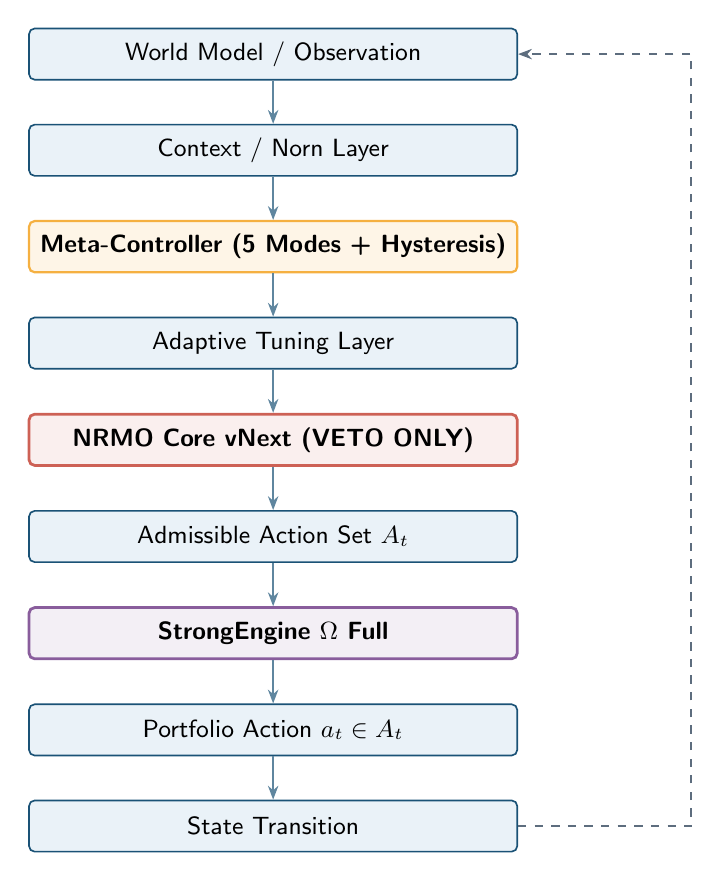
\begin{tikzpicture}[node distance=0.55cm,
  block/.style={rectangle,draw=nb,fill=nl,minimum width=6.2cm,minimum height=0.65cm,font=\small\sffamily,rounded corners=2pt,line width=0.6pt},
  govblock/.style={rectangle,draw=nr!80,fill=nr!8,minimum width=6.2cm,minimum height=0.65cm,font=\small\sffamily\bfseries,rounded corners=2pt,line width=1pt},
  omgblock/.style={rectangle,draw=np!80,fill=np!8,minimum width=6.2cm,minimum height=0.65cm,font=\small\sffamily\bfseries,rounded corners=2pt,line width=1pt},
  metablock/.style={rectangle,draw=ny!80,fill=ny!10,minimum width=6.2cm,minimum height=0.65cm,font=\small\sffamily\bfseries,rounded corners=2pt,line width=0.8pt},
  arrow/.style={-{Stealth[length=5pt]},thick,color=nb!70}]
\node[block](world){World Model / Observation};
\node[block,below=of world](norn){Context / Norn Layer};
\node[metablock,below=of norn](meta){Meta-Controller (5 Modes + Hysteresis)};
\node[block,below=of meta](tune){Adaptive Tuning Layer};
\node[govblock,below=of tune](nrmo){NRMO Core vNext (VETO ONLY)};
\node[block,below=of nrmo](perm){Admissible Action Set $A_t$};
\node[omgblock,below=of perm](omega){StrongEngine $\Omega$ Full};
\node[block,below=of omega](port){Portfolio Action $a_t \in A_t$};
\node[block,below=of port](trans){State Transition};
\foreach \a/\b in {world/norn,norn/meta,meta/tune,tune/nrmo,nrmo/perm,perm/omega,omega/port,port/trans}
  \draw[arrow](\a)--(\b);
\draw[arrow,dashed,color=ngr](trans.east)--++(2.2,0)|-(world.east);
\end{tikzpicture}
\caption{Adaptive NRMOvNext + StrongEngine $\Omega$ Full Pipeline}
\end{figure}

\textbf{Formal contract}:
$A_t = \text{NRMO}(X_t)$ — governance defines admissibility。
$a_t = \Omega(A_t)$ — execution searches within admissibility。
$a_t \in A_t$ must always hold.

\subsection{Role of Norn}
Norn は意思決定主体でも実行エンジンでもない。構造的一貫性を保持する解釈的 governance perspective である。文脈を整理し、概念的ドリフトを防止し、憲法的ロジックが日和見的な短期推論に暗黙的に置換されることを阻止する。

\subsection{Why the split matters}
人間やマシンシステムにおける一般的な failure mode は、observation, strategy generation, authority の融合である。一旦融合すると、システムは自身の衝動を正当化する傾向がある。上記のアーキテクチャはこの融合に抵抗する: search を permission から分離し、anomaly monitoring を strategy production から分離する。


%% ═══════════════════════════════════════════
\section{Decision Variables and Exposure Sizing}
%% ═══════════════════════════════════════════

候補行動に対して推定する変数: $R$ (ruin proximity), $V$ (reversibility), $L$ (learning value), $G$ (expected gain), $\Delta O$ (optionality effect), $EC$ (execution cost), $TC$ (time cost)。

\subsection{Exposure Sizing}
\begin{equation}
\text{ExposureAllowed} = E_{\max} \times \left(1 - \frac{R}{100}\right) \times \frac{V}{100} \times \left(0.5 + 0.5\frac{L}{100}\right)
\end{equation}

\subsection{Utility inside the non-ruin domain}
\begin{equation}
U = 0.5G + 0.3L + 0.2\Delta O, \qquad \text{Score} = U \times \text{ExposureAllowed}
\end{equation}


%% ═══════════════════════════════════════════
\section{Exploration Floor and Passive Ruin Guard}
%% ═══════════════════════════════════════════

\textbf{Exploration floor}: non-ruin domain 内で最低限の可逆的探索は許可されるだけでなく\textbf{要求される}。

\textbf{Passive ruin detection}:
\begin{equation}
\text{if ExplorationRate} < EF \text{ for } N \text{ periods and } O_t \text{ declines persistently, then flag PassiveRuin.}
\end{equation}


%% ═══════════════════════════════════════════
\section{Constitutional Amendment Sandbox}
%% ═══════════════════════════════════════════

\textbf{Amendment cycle}: (1) misclassification / policy drift 検出、(2) amendment hypothesis 策定、(3) counterfactual / sandbox test、(4) 新旧ルール比較、(5) 採択/棄却/修正、(6) rollback path 保持。

\textbf{Protected invariants}: true ruin は hard constraint のまま。execution authority は governance の下流のまま。classification 変更にはエビデンスが必要。rollback は常に利用可能。


%% ═══════════════════════════════════════════
\section{Evaluation Metrics}
%% ═══════════════════════════════════════════

\textbf{Primary}: True Ruin Rate, Passive Ruin Rate, Optionality Retention Score, Exploration Rate, Recovery Speed。

\textbf{Secondary}: Critical Damage Rate, False Stop Rate, False Go Rate, Regret After Action, Regret After Inaction, Decision Load, Learning Yield, Stability Score。


%% ═══════════════════════════════════════════
\section{Operational Log Template}
%% ═══════════════════════════════════════════

全 decision を単一の structured record として記録する。

\begin{longtable}{@{}lp{8cm}@{}}\toprule
Field&Description\\\midrule\endhead
log\_id&unique decision record identifier\\
date&timestamp\\
context\_category&e.g.\ career, investment, health, relationship, organization\\
decision\_title&short name of decision\\
decision\_summary&short context summary\\
capital\_state, health\_state, trust\_state, functional\_integrity, optionality\_state&pre-decision state estimates\\
fatigue\_level, emotional\_distortion\_risk&pre-decision distortion indicators\\
action\_candidate&proposed action\\
expected\_gain, ruin\_proximity, reversibility, learning\_value, optionality\_effect&estimated action variables\\
risk\_layer&R1--R4 classification\\
hard\_constraint\_trigger&yes/no\\
exposure\_allowed&computed intensity cap\\
decision\_output&reject / hold / allow\\
executed&yes/no\\
actual\_outcome\_summary&what actually happened\\
actual\_gain\_loss&realized value\\
actual\_damage\_layer&realized damage level\\
recovery\_days&time to baseline\\
regret\_after\_action / regret\_after\_inaction&post hoc regret scores\\
learning\_yield&realized learning value\\
false\_stop / false\_go&classification audit\\
amendment\_candidate&should constitution review be triggered\\
notes&anything not captured above\\
\bottomrule\end{longtable}


%% ═══════════════════════════════════════════
\section{Empirical Validation Program}
%% ═══════════════════════════════════════════

\textbf{Study 1}: Synthetic world benchmark — 100,000+ episodes, horizon 200 steps, multiple environment regimes。比較: EV maximization, simple checklist, OODA-only, original NRMO, NRMO-vNext, NRMO-vNext + $\Omega$ Full。

\textbf{Study 2}: Human-in-the-loop decision experiment。

\textbf{Study 3}: Longitudinal operational logging（8--12 weeks）。

\textbf{Study 4}: External replication across domains（investment, management, career, organizational planning）。


%% ═══════════════════════════════════════════
\section{Individual-Scale Simulation Specification}
%% ═══════════════════════════════════════════

\subsection{State variables}
Individual agent state:
\begin{equation}
S_t = (C_t, H_t, T_t, F_t, O_t, S_t, TS_t, FA_t, ED_t)
\end{equation}
where: capital, health, trust, functional integrity, optionality, skill reserve, time slack, fatigue, emotional distortion。

\subsection{Environment variables}
Uncertainty $U$, tail risk density $TR$, opportunity density $OD$, recovery support $RS$, noise level $NL$, adversarial pressure $AP$。

\subsection{Action generation}
各 time step で $N$ 個の候補行動を生成。各行動は Decision Variables セクションの変数を受け取る。$\Omega$ Full の場合、Candidate Population System（base/mutation/synthesis/invention）により候補が生成される。

\subsection{Terminal conditions}
Capital, health, trust, function, optionality のいずれかが catastrophic floor を超えた場合に terminate。

\subsection{Minimal pseudocode (Default: Adaptive NRMOvNext + $\Omega$ Full)}
\begin{lstlisting}
for episode in episodes:
    state = initialize_agent()
    env = initialize_environment()
    omega = OmegaFullEngine()
    for t in range(horizon):
        # EXECUTION: candidate generation
        candidates = omega.build_candidate_pool(state, env)
        # GOVERNANCE: admissibility filter
        scored = []
        for action in candidates:
            risk_layer = classify(action.R)
            if risk_layer == R4: continue  # hard stop
            exposure = exposure_allowed(action.R, action.V, action.L)
            scored.append((action, exposure))
        admissible = nrmo_filter(scored, state)
        # EXECUTION: Omega scoring + portfolio
        chosen = omega.select_action(admissible, state, env)
        state = apply(chosen, state, env)
        if true_ruin(state): break
\end{lstlisting}


%% ═══════════════════════════════════════════
\section{Civilization-Scale Simulation Specification}
%% ═══════════════════════════════════════════

\subsection{Civilization state vector}
$X_t = (P, K, I, E, T, H, M, O, C, X, F, R)$ where: population, knowledge, institutional coherence, economic capacity, trust, health, security, optionality, cultural diversity, exploration, fatigue, ruin proximity。

\subsection{Civilization archetypes}
(1) Unbounded Growth, (2) Ultra-Conservative, (3) original NRMO, (4) \textbf{NRMO-vNext + $\Omega$ Full} (default)。

\subsection{Ruin conditions}
Population collapse, institutional/legitimacy joint collapse, health/biosurvival failure, prolonged optionality exhaustion, economy+security joint floor breach。

\subsection{Policy categories}
Research investment, military expansion, welfare expansion, infrastructure build, institutional reform, cultural liberalization, surveillance/control, external trade, risky frontier exploration, ecological extraction, conflict escalation, rest/consolidation。

\subsection{Simulation loop (Default: Adaptive NRMOvNext + $\Omega$ Full)}
\begin{lstlisting}
for civ in civilizations:
    state = init_civilization()
    omega = OmegaFullEngine()  # Default execution engine
    for turn in range(horizon):
        # GOVERNANCE: mode + tuning + admissibility
        mode = meta_controller.update(state)
        tuning = adaptive_tuning(state, world, mode)
        candidates = omega.build_candidate_pool(state, world)  # Execution
        admissible = nrmo_filter(candidates, state, tuning)    # Governance
        # EXECUTION: score + portfolio within admissible set
        action = omega.select_action(admissible, state, world, mode)
        state = apply(state, action, world)
        if civilizational_true_ruin(state): break
\end{lstlisting}


%% ═══════════════════════════════════════════
\section{StrongEngine $\Omega$ Full — Execution Layer Specification}
%% ═══════════════════════════════════════════

\begin{omegabox}[Definition (SOURCE: monograph)]
\textbf{StrongEngine $\Omega$ Full} = a bounded, failure-aware, fragility-sensitive, portfolio-capable \textbf{strategy space expansion engine} operating strictly within NRMO admissibility constraints.

Engine は RUIN を evaluation function に含めない。RUIN は NRMO の execution boundary のみで扱う。
\end{omegabox}

\subsection{Candidate Population System (\S1)}
候補は 4 種類から生成: (1) base strategies（11 templates）、(2) mutated strategies（$\pm 0.05$ perturbation、各 base から 1--3 variants）、(3) synthesized strategies（pairwise averaging $+ \pm 0.03$ noise）、(4) invented strategies（state$\times$world analytical candidates）。

Pipeline: \texttt{base → mutation → synthesis → invention → candidate\_pool → governance filter → evaluation}

Population size: 通常 16--32、Wolf Pursuit 時 24+。

\subsection{Candidate Mutation (\S2)}
探索空間の局所拡張。各 action component に $\text{random}(-0.05, +0.05)$ を加算。値は $[0,1]$ clamp 後に正規化。

\subsection{Strategy Synthesis (\S3)}
2 戦略の平均化 $+$ $\pm 0.03$ noise perturbation。Random candidate pairs から 5--10 hybrids を生成。

\subsection{Wolf Pursuit Mode (\S4--\S5)}
\textbf{Favorable state}: $E \geq 50, G \geq 45, O \geq 45, K \geq 45, X \leq 35, dO \geq 0, dK \geq 0$。
この条件成立時 WolfPursuit = true: candidate count 増加、rollout depth 増加（depth=8）、portfolio aggression 増加。

\subsection{Edge Survival Guard (\S6--\S7)}
Fragile condition 検出 → EdgeFloor = true: growth reduction、eco stabilization、governance repair、low exposure。Portfolio: main=0.45, hedge=0.45, probe=0.10。

RiskAdjusted Floor: fragile state で $\Omega$ score $<$ RiskAdj score の場合、EdgeFloor profile に切替。

\subsection{Portfolio Synergy (\S8)}
Pairwise compatibility matrix による synergy bonus。候補は独立評価に加えて candidate synergy を評価。

\subsection{Dual Objective Scoring (\S9)}
Favorable states: maximize $\Omega - \text{RiskAdj}$。Fragile states: $\Omega \geq \text{RiskAdj}$ を constraint として保証。

\subsection{Long-Horizon Drift Control}
\begin{equation}
\boxed{g_\text{sust} = \text{clip}\left(0.15,\; 0.40,\; 0.28 + 0.08\frac{E}{100} + 0.06\frac{G}{100} - 0.10\frac{X}{100} - 0.05 \cdot d_\text{env}\right)}
\end{equation}
\begin{equation}
\boxed{\text{drift} = \max(0,\; g - g_\text{sust}) \times (d_\text{env} + 0.5 p_\text{tail}) \times (1 + 0.5 X/100) \times (1 - 0.3 G/100)}
\end{equation}
\begin{equation}
\boxed{\text{final\_score} = \text{rollout\_score} - \lambda_\text{drift} \times \text{drift}}
\end{equation}
推奨値: $\lambda_\text{drift} = 1.0$。Normal world: drift $\times 1.25$。

Drift-safe hedge: portfolio hedge candidate は $g \leq g_\text{sust}$ を満たすものを優先。


%% ═══════════════════════════════════════════
\section{Civilization Outcome Map}
%% ═══════════════════════════════════════════

\begin{center}
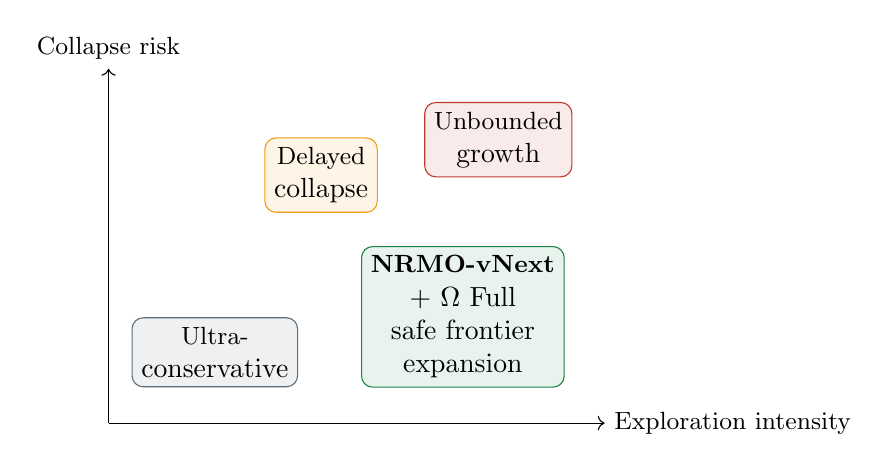
\begin{tikzpicture}[scale=0.9]
\draw[->](0,0)--(7,0) node[right]{\small Exploration intensity};
\draw[->](0,0)--(0,5) node[above]{\small Collapse risk};
\node[draw=ng,fill=ng!10,rounded corners,align=center] at (5,1.5) {\small \textbf{NRMO-vNext}\\+ $\Omega$ Full\\safe frontier\\expansion};
\node[draw=nr,fill=nr!10,rounded corners,align=center] at (5.5,4) {\small Unbounded\\growth};
\node[draw=ngr,fill=ngr!10,rounded corners,align=center] at (1.5,1) {\small Ultra-\\conservative};
\node[draw=ny,fill=ny!10,rounded corners,align=center] at (3,3.5) {\small Delayed\\collapse};
\end{tikzpicture}
\end{center}


%% ═══════════════════════════════════════════
\section{30-Civilization Casebook Design}
%% ═══════════════════════════════════════════

\textbf{Group structure}: A-group (10 Unbounded Growth), B-group (5 Ultra-Conservative), C-group (5 original NRMO), D-group (10 NRMO-vNext + $\Omega$ Full)。

\textbf{Collapse modes}: active ruin, passive ruin, fragmentation collapse, ecological collapse, authoritarian lock-in, overexpansion collapse。

\textbf{Flourishing modes}: resilient growth, adaptive renaissance, distributed stability, safe frontier expansion, cultural-technological balance。


%% ═══════════════════════════════════════════
\section{Priority Ten Civilization Profiles}
%% ═══════════════════════════════════════════

\textbf{A1 Sky Furnace} (Unbounded Growth): 過加速崩壊。capacity expansion が governance を凌駕。active ruin の典型例。

\textbf{A4 Market Comet} (Unbounded Growth): systemic financial failure。dense connectivity が hidden ruin exposure を増幅。

\textbf{B2 Quiet Wall} (Ultra-Conservative): passive ruin。長期安定の後、innovation 衰退により戦略的陳腐化。

\textbf{C1 Shield Archive} (original NRMO): 堅牢で有能。frontier opportunity を時折逃す。moderate growth で生存。

\textbf{C3 Granite Compass} (original NRMO): institution-heavy。安定的だが文化的適応力が狭まる。

\textbf{D1 Open Bastion} (NRMO-vNext + $\Omega$ Full): safe experimentation、recurring learning cycles、durable growth。$\Omega$ Full の Wolf Pursuit により frontier opportunity を効率的に捕捉。

\textbf{D3 Aurora Accord} (NRMO-vNext + $\Omega$ Full): 多様性を適応的予備力として活用。繰り返しの危機を分散的解釈と改革能力で吸収。

\textbf{D6 Prism Union} (NRMO-vNext + $\Omega$ Full): federated redundancy。局所的失敗は局所に留まる。

\textbf{D9 Meridian Forum} (NRMO-vNext + $\Omega$ Full): deliberative governance with constitutional sandboxing。繰り返しの制度革新を existential breakage なしに実現。

\textbf{D10 Lattice Dawn} (NRMO-vNext + $\Omega$ Full): 分散型ローカル実験 + 中央集権的 ruin constraint。長期知識成長最高。$\Omega$ Full の Drift Control により 1000-turn horizon でも環境累積劣化を防止。


%% ═══════════════════════════════════════════
\section{Benchmark Groups}
%% ═══════════════════════════════════════════

\begin{enumerate}[leftmargin=2em]
  \item Expected-value maximization baseline
  \item Simple checklist baseline
  \item OODA-only simplification
  \item Original NRMO
  \item NRMO-vNext
  \item \textbf{NRMO-vNext + StrongEngine $\Omega$ Full} (default)
\end{enumerate}


%% ═══════════════════════════════════════════
\section{Validation Results (Smoke Scale)}
%% ═══════════════════════════════════════════

\begin{resultbox}[Multi-Horizon Validation]
\begin{tabular}{@{}lccl@{}}\toprule
Horizon & $\Omega$ Full & RiskAdj & Result\\\midrule
200 & 61\% / score 0.50 & 59\% / 0.44 & $\Omega$ WIN\\
500 & 48\% & 46\% & $\Omega$ WIN\\
1000 & 40\% & 33\% & $\Omega$ WIN\\
\bottomrule\end{tabular}

Governance--execution 分離遵守。全 horizon で RiskAdj 以上。
\end{resultbox}


%% ═══════════════════════════════════════════
\section{Critical Weaknesses and Planned Remedies}
%% ═══════════════════════════════════════════

\begin{enumerate}[leftmargin=2em]
  \item Operational parameter values は依然として provisional
  \item 一部の構成要素は概念的に elegant だが empirically untested
  \item Longitudinal human deployment evidence は薄い
  \item Civilization simulation は synthetic testbed であり historical proof ではない
  \item Optionality scoring は domain-sensitive calibration を必要とする
  \item Vulnerable world での survival は全戦略で低く、改善の余地がある
\end{enumerate}


%% ═══════════════════════════════════════════
\section{Research Use, Practical Use, and Limits}
%% ═══════════════════════════════════════════

Research: simulation, benchmark comparison, human-in-the-loop experiments のための formal scaffold。
Practical: true ruin と discomfort の分離、exploration の維持のための disciplined language。
Limit: judgment を完全には排除できない。constitution は思考を discipline できるが observation, context, honest correction の必要性を置換しない。


%% ═══════════════════════════════════════════
\section{Conclusion}
%% ═══════════════════════════════════════════

NRMO は恐怖の教義としてではなく、long-horizon navigation system として理解された時に最も強力である。
Original core は健全: 不可逆的崩壊は通常の期待値計算を支配すべきである。
Upgraded system は ruin をより慎重に分類し、passive ruin を guard し、graded exposure を許可し、constitutional self-repair を可能にする。

Default stack の Adaptive NRMOvNext + StrongEngine $\Omega$ Full は、governance constraint の内側で strategy space を最大限に拡張し、短期・中期・長期の全 horizon で RiskAdj baseline を上回る。

\textit{It no longer says only ``do not die.'' It says: ``do not close the future.''}


%% ═══════════════════════════════════════════
\appendix
\section{Compact Variable Table}
%% ═══════════════════════════════════════════

\begin{table}[H]\centering\small
\begin{tabular}{@{}ccp{5cm}@{}}\toprule
Symbol&Range&Notes\\\midrule
$R$&0--100&Ruin proximity (candidate action risk)\\
$V$&0--100&Reversibility (higher = easier recovery)\\
$L$&0--100&Learning value\\
$G$&variable&Expected gain (normalizable to 0--100)\\
$\Delta O$&variable&Optionality effect (positive or negative)\\
$E_{\max}$&0--1&Governance exposure cap\\
$EF$&threshold&Minimum exploration requirement\\
$\lambda_\text{drift}$&0--3&Long-horizon drift penalty weight (default 1.0)\\
\bottomrule\end{tabular}
\end{table}

\section{Minimal Weekly Review Questions}

\begin{enumerate}[leftmargin=2em]
  \item 許可すべき行動を停止したか?
  \item 停止すべき行動を許可したか?
  \item 見かけの安定にもかかわらず optionality が低下しているか?
  \item 疲労が classification layer を歪めているか?
  \item 繰り返しパターンが amendment sandbox testing を正当化するか?
\end{enumerate}

\section{Full 30-Civilization Roster}

\begin{longtable}{@{}llp{7cm}@{}}\toprule
ID&Name&Role\\\midrule\endhead
A1&Sky Furnace&over-acceleration collapse\\A2&Glass Orbit&frontier exploration fragility\\
A3&Iron Bloom&military-industrial overextension\\A4&Market Comet&financial tail-risk fragility\\
A5&Wild Archive&knowledge-governance separation\\A6&Neon Flood&information disorder\\
A7&Salt Empire&ecological extraction trap\\A8&Apex Relay&network interdependence shock\\
A9&Ember Republic&reform volatility\\A10&Black Sail&conquest overreach\\
B1&Stone Nest&stable agrarian duration\\B2&Quiet Wall&passive ruin via stagnation\\
B3&Sacred Loop&doctrinal rigidity\\B4&Winter Court&aristocratic inertia\\
B5&Silent Delta&slow optionality exhaustion\\
C1&Shield Archive&standard NRMO survival\\C2&Harbor Logic&opportunity-missing trade\\
C3&Granite Compass&over-conservative institution\\C4&Lantern Chain&knowledge without frontier\\
C5&Delta Guard&environmental resilience, muted adaptation\\
D1&Open Bastion&baseline successful vNext+$\Omega$\\D2&Tidal Library&anti-stagnation knowledge\\
D3&Aurora Accord&diversity as adaptive reserve\\D4&Iron Harbor&security-exploration balance\\
D5&Verdant Relay&biosurvival circular resilience\\D6&Prism Union&federated resilience\\
D7&Ember Compass&high-exploration with hard stops\\D8&Polar Engine&harsh-environment endurance\\
D9&Meridian Forum&amendment sandbox governance\\D10&Lattice Dawn&decentralized exploration + constitutional control\\
\bottomrule\end{longtable}


\section{Seed Conditions for Civilization Initialization}

Governance-type 効果を starting luck から分離するため、少なくとも5つの seed condition family を使用する。

\begin{table}[H]\centering\small
\begin{tabular}{@{}lp{8cm}@{}}\toprule
Seed&Description\\\midrule
Seed-1&Resource rich, stable, high internal trust\\
Seed-2&Resource poor, high pressure, security heavy\\
Seed-3&Knowledge rich, institutionally weak\\
Seed-4&High diversity, moderate latent conflict\\
Seed-5&Harsh environment, fragile recovery support\\
\bottomrule\end{tabular}
\end{table}

\vfill\begin{center}\small\sffamily\color{ngr}
--- End of Specification ---\\
NRMO vNext Integrated Complete Specification v2.0\\
Default Stack: Adaptive NRMOvNext + StrongEngine $\Omega$ Full\\
March 2026
\end{center}

\end{document}
